\documentclass[12pt,a4paper]{article}
\usepackage{amsmath, amssymb, geometry, booktabs, xcolor, hyperref,
            listings, pgfplots, tcolorbox, enumitem, fancyhdr, tikz, array}
\usepgfplotslibrary{fillbetween}
\geometry{margin=2.5cm}
\pgfplotsset{compat=1.18}
\tcbuselibrary{skins, breakable}

\newtcolorbox{curiositybox}[1]{colback=yellow!10, colframe=orange!80, title=#1, breakable}
\newtcolorbox{infobox}[1]{colback=blue!5, colframe=blue!60, title=#1, breakable}
\newtcolorbox{mistakebox}[1]{colback=red!5, colframe=red!60, title=#1, breakable}
\newtcolorbox{learnbox}[1]{colback=green!5, colframe=green!60, title=#1, breakable}

\pagestyle{fancy}
\fancyhf{}
\lhead{Matrix Fundamentals}
\rhead{Unit 1 --- LAC}
\cfoot{\thepage}

\title{\textbf{Matrix Fundamentals: Definition, Types, Operations, Transpose, Inverse, Symmetric \& Skew-Symmetric Matrices} \\ \large Unit 1 --- Matrix Algebra and Linear Systems}
\author{Department of Mathematics}
\date{\today}

\begin{document}
\maketitle
\tableofcontents
\newpage

%===========================================================
\section{Real-World Engineering Hook}
%===========================================================

\begin{curiositybox}{Why Should an Engineer Care?}
Imagine a structural engineer analysing a steel truss bridge. Every joint in the bridge has forces acting on it in multiple directions. The engineer stores all these forces in a \textbf{matrix} --- a rectangular grid of numbers. To find whether the bridge will hold its load, they must \emph{add} force matrices from different load cases, \emph{multiply} transformation matrices to rotate coordinate systems, and \emph{invert} stiffness matrices to solve for displacements. A single mistake in matrix multiplication or an incorrect inverse can predict that a bridge is safe when it is not --- with catastrophic consequences.

Matrix algebra is not just abstract mathematics. It is the computational backbone of modern engineering:
\begin{itemize}
  \item \textbf{Google PageRank}: The importance of every web page is an eigenvector of a gigantic matrix. The entire internet ranking depends on matrix operations.
  \item \textbf{JPEG Image Compression}: Your photographs are stored as matrices of pixel values. The Discrete Cosine Transform --- a matrix multiplication --- compresses them to a fraction of their original size.
  \item \textbf{3D Computer Graphics}: Every rotation, scaling, and translation of a 3D object on your screen is a $4\times 4$ matrix multiplication applied thousands of times per frame.
  \item \textbf{Finite Element Analysis (FEA)}: Simulating stress in a car body or an aircraft wing requires assembling and inverting matrices with millions of entries.
\end{itemize}
Understanding matrices deeply --- their types, their operations, and their properties --- is the first and most critical step in any engineer's mathematical education.
\end{curiositybox}

%===========================================================
\section{Why This Topic Exists --- Theory vs Real-World Impact}
%===========================================================

\begin{center}
\begin{tabular}{@{}p{5.5cm}p{9cm}@{}}
\toprule
\textbf{Theoretical Concept} & \textbf{Engineering Application / Consequence of Misunderstanding} \\
\midrule
Matrix Definition, Order, Notation & Incorrectly indexing a stiffness matrix entry $a_{ij}$ vs $a_{ji}$ places a force in the wrong direction, causing wrong structural predictions. \\
\addlinespace
Types of Matrices & Misidentifying a matrix as invertible when it is nilpotent leads to attempting a division by zero equivalent in circuit analysis. \\
\addlinespace
Matrix Operations & Non-commutativity of multiplication ($AB \neq BA$) matters critically in robotics: applying rotation before translation gives a different robot pose than translation before rotation. \\
\addlinespace
Transpose of a Matrix & The reversal rule $(AB)^T = B^T A^T$ is used when converting between row-vector and column-vector formulations in signal processing and control systems. \\
\addlinespace
Inverse of a Matrix & Inverting the stiffness matrix in FEA gives nodal displacements. Using the adjugate formula correctly is essential; an error in any of the 9 cofactors corrupts the entire solution. \\
\addlinespace
Symmetric Matrices & The stiffness matrix in structural engineering is always symmetric. Exploiting symmetry halves storage and computation time in large simulations. \\
\addlinespace
Skew-Symmetric Matrices & Angular velocity tensors in robotics are skew-symmetric. Misidentifying them as general matrices discards the constraint that diagonal entries must be zero. \\
\bottomrule
\end{tabular}
\end{center}

\begin{learnbox}{Core Motivation}
Matrices are the language of linear transformations --- mastering all types and operations is non-negotiable for every engineer.
\end{learnbox}

%===========================================================
\section{Intuition First and Mathematical Definitions}
%===========================================================

\subsection{Matrices --- Definition and Notation}

Think of a matrix as a spreadsheet of numbers arranged in rows and columns. Just as a spreadsheet cell is addressed by its row and column number, each entry of a matrix is identified by two indices. The beauty of this notation is that it lets us talk about any entry in any matrix of any size using a single, consistent language.

\begin{infobox}{Matrix: Definition and Notation}
A \textbf{matrix} is a rectangular array of numbers (real or complex) arranged in $m$ horizontal \emph{rows} and $n$ vertical \emph{columns}, written as:
\[
A = \begin{pmatrix} a_{11} & a_{12} & \cdots & a_{1n} \\ a_{21} & a_{22} & \cdots & a_{2n} \\ \vdots & \vdots & \ddots & \vdots \\ a_{m1} & a_{m2} & \cdots & a_{mn} \end{pmatrix}
\]
\textbf{Order (Size):} The matrix $A$ above has order $m \times n$ (read: $m$ by $n$). The first number is always the number of rows; the second is the number of columns.

\textbf{Element Notation:} The element in row $i$ and column $j$ is denoted $a_{ij}$. The first subscript is the \emph{row index}, the second is the \emph{column index}.

\textbf{Compact Notation:} We write $A = [a_{ij}]_{m \times n}$ or simply $A = [a_{ij}]$.

\textbf{Special Index:} Elements where $i = j$ (i.e., $a_{11}, a_{22}, \ldots$) lie on the \textbf{main diagonal}.
\end{infobox}

\textbf{Worked Example 1.1 --- Identifying Elements by Position:}

Let $A = \begin{pmatrix} 5 & -3 & 7 & 2 \\ 0 & 8 & -1 & 4 \\ 6 & 1 & 3 & -9 \end{pmatrix}$.

\begin{enumerate}[label=(\alph*)]
  \item \textbf{Order of $A$:} $A$ has 3 rows and 4 columns, so order = $3 \times 4$. Since $m \neq n$, $A$ is rectangular (not square).
  \item \textbf{Element $a_{23}$:} Row 2, Column 3. Counting across row 2: $0, 8, \mathbf{-1}, 4$. So $a_{23} = -1$.
  \item \textbf{Element $a_{31}$:} Row 3, Column 1. First element of row 3: $\mathbf{6}$. So $a_{31} = 6$.
  \item \textbf{Element in row 2, column 4:} That is $a_{24}$. Row 2: $0, 8, -1, \mathbf{4}$. So $a_{24} = 4$.
  \item \textbf{Main diagonal:} Elements $a_{11} = 5$, $a_{22} = 8$, $a_{33} = 3$ (only 3 diagonal entries since min$(m,n) = 3$).
\end{enumerate}

\begin{learnbox}{Row First, Column Second}
$a_{ij}$ means row $i$, column $j$ --- \emph{always row first, column second}. Remember: \textbf{R}ow before \textbf{C}olumn, just like \textbf{RC} in a circuit (Row-Column).
\end{learnbox}

%-----------------------------------------------------------
\subsection{Types of Matrices}

Matrices come in many special flavours, each with algebraic conditions that unlock powerful properties. Learning to recognise types quickly is like knowing the difference between a transistor and a resistor --- the same object (a component / a matrix), but with radically different behaviour.

\begin{infobox}{Types of Matrices --- Complete Classification}
\textbf{1. Square Matrix:} $m = n$ (same number of rows and columns). \\[2pt]
\textbf{2. Rectangular Matrix:} $m \neq n$. \\[2pt]
\textbf{3. Row Matrix (Row Vector):} Only one row, $m = 1$. Example: $\begin{pmatrix} 1 & 2 & 3 \end{pmatrix}$. \\[2pt]
\textbf{4. Column Matrix (Column Vector):} Only one column, $n = 1$. Example: $\begin{pmatrix} 4 \\ 5 \\ 6 \end{pmatrix}$. \\[2pt]
\textbf{5. Null (Zero) Matrix:} All entries are zero. Denoted $O$ or $\mathbf{0}$. \\[2pt]
\textbf{6. Identity Matrix:} Square matrix with $a_{ii} = 1$ and $a_{ij} = 0$ for $i \neq j$. Denoted $I_n$. Example: $I_2 = \begin{pmatrix} 1 & 0 \\ 0 & 1 \end{pmatrix}$. \\[2pt]
\textbf{7. Diagonal Matrix:} Square matrix where $a_{ij} = 0$ for all $i \neq j$. Example: $\begin{pmatrix} 3 & 0 \\ 0 & 7 \end{pmatrix}$. \\[2pt]
\textbf{8. Scalar Matrix:} Diagonal matrix where all diagonal entries are equal. Example: $\begin{pmatrix} 5 & 0 \\ 0 & 5 \end{pmatrix}$. \\[2pt]
\textbf{9. Upper Triangular Matrix:} $a_{ij} = 0$ whenever $i > j$ (all entries below the diagonal are zero). Example: $\begin{pmatrix} 1 & 2 & 3 \\ 0 & 4 & 5 \\ 0 & 0 & 6 \end{pmatrix}$. \\[2pt]
\textbf{10. Lower Triangular Matrix:} $a_{ij} = 0$ whenever $i < j$ (all entries above the diagonal are zero). Example: $\begin{pmatrix} 1 & 0 & 0 \\ 2 & 3 & 0 \\ 4 & 5 & 6 \end{pmatrix}$. \\[2pt]
\textbf{11. Symmetric Matrix:} $A^T = A$, i.e., $a_{ij} = a_{ji}$ for all $i, j$. Must be square. Example: $\begin{pmatrix} 1 & 2 \\ 2 & 5 \end{pmatrix}$. \\[2pt]
\textbf{12. Skew-Symmetric Matrix:} $A^T = -A$, i.e., $a_{ij} = -a_{ji}$ for all $i, j$. Diagonal entries must be zero. Example: $\begin{pmatrix} 0 & 3 \\ -3 & 0 \end{pmatrix}$. \\[2pt]
\textbf{13. Orthogonal Matrix:} $A^T A = I$, equivalently $A^{-1} = A^T$. Preserves lengths and angles. Example: $\begin{pmatrix} \cos\theta & -\sin\theta \\ \sin\theta & \cos\theta \end{pmatrix}$. \\[2pt]
\textbf{14. Idempotent Matrix:} $A^2 = A$. These are projection matrices --- applying the transformation twice is the same as applying it once. All eigenvalues of an idempotent matrix belong to the set $\{0, 1\}$. Example: $\begin{pmatrix} 1 & 0 \\ 0 & 0 \end{pmatrix}$. \\[2pt]
\textbf{15. Involutory Matrix:} $A^2 = I$. These are reflection matrices --- applying the transformation twice returns to the identity. All eigenvalues of an involutory matrix belong to $\{-1, +1\}$. Example: $\begin{pmatrix} 1 & 0 \\ 0 & -1 \end{pmatrix}$. \\[2pt]
\textbf{16. Nilpotent Matrix:} $A^k = O$ for some positive integer $k$. The smallest such $k$ is called the \emph{index of nilpotency}. All eigenvalues of a nilpotent matrix equal $0$. Example (index 2): $\begin{pmatrix} 0 & 1 \\ 0 & 0 \end{pmatrix}$ since $\begin{pmatrix} 0 & 1 \\ 0 & 0 \end{pmatrix}^2 = \begin{pmatrix} 0 & 0 \\ 0 & 0 \end{pmatrix}$.
\end{infobox}

\textbf{Worked Example 1.2 --- Classifying Six Matrices:}

Classify each of the following matrices with full justification.

\medskip
\textbf{(a) Idempotent:} $P = \begin{pmatrix} 1 & 0 \\ 0 & 0 \end{pmatrix}$.

Compute $P^2$:
\[
P^2 = \begin{pmatrix} 1 & 0 \\ 0 & 0 \end{pmatrix}\begin{pmatrix} 1 & 0 \\ 0 & 0 \end{pmatrix} = \begin{pmatrix} 1\cdot1+0\cdot0 & 1\cdot0+0\cdot0 \\ 0\cdot1+0\cdot0 & 0\cdot0+0\cdot0 \end{pmatrix} = \begin{pmatrix} 1 & 0 \\ 0 & 0 \end{pmatrix} = P.
\]
Since $P^2 = P$, \textbf{$P$ is Idempotent}. (It projects every vector onto the $x$-axis.)

\medskip
\textbf{(b) Involutory:} $R = \begin{pmatrix} 1 & 0 \\ 0 & -1 \end{pmatrix}$.

Compute $R^2$:
\[
R^2 = \begin{pmatrix} 1 & 0 \\ 0 & -1 \end{pmatrix}\begin{pmatrix} 1 & 0 \\ 0 & -1 \end{pmatrix} = \begin{pmatrix} 1\cdot1+0\cdot0 & 1\cdot0+0\cdot(-1) \\ 0\cdot1+(-1)\cdot0 & 0\cdot0+(-1)\cdot(-1) \end{pmatrix} = \begin{pmatrix} 1 & 0 \\ 0 & 1 \end{pmatrix} = I.
\]
Since $R^2 = I$, \textbf{$R$ is Involutory}. (It reflects every vector in the $x$-axis.)

\medskip
\textbf{(c) Nilpotent (index 2):} $N = \begin{pmatrix} 0 & 2 \\ 0 & 0 \end{pmatrix}$.

Compute $N^2$:
\[
N^2 = \begin{pmatrix} 0 & 2 \\ 0 & 0 \end{pmatrix}\begin{pmatrix} 0 & 2 \\ 0 & 0 \end{pmatrix} = \begin{pmatrix} 0\cdot0+2\cdot0 & 0\cdot2+2\cdot0 \\ 0\cdot0+0\cdot0 & 0\cdot2+0\cdot0 \end{pmatrix} = \begin{pmatrix} 0 & 0 \\ 0 & 0 \end{pmatrix} = O.
\]
Since $N^2 = O$, \textbf{$N$ is Nilpotent with index 2}.

\medskip
\textbf{(d) Diagonal:} $D = \begin{pmatrix} 4 & 0 & 0 \\ 0 & -2 & 0 \\ 0 & 0 & 7 \end{pmatrix}$.

All off-diagonal entries are zero: $d_{12}=d_{13}=d_{21}=d_{23}=d_{31}=d_{32}=0$. Diagonal entries are not all equal. \textbf{$D$ is a Diagonal matrix} (not scalar since $4 \neq -2 \neq 7$).

\medskip
\textbf{(e) Upper Triangular:} $U = \begin{pmatrix} 3 & 5 & 1 \\ 0 & 2 & 4 \\ 0 & 0 & 6 \end{pmatrix}$.

Check all entries below the main diagonal: $u_{21}=0$, $u_{31}=0$, $u_{32}=0$. All zero. \textbf{$U$ is Upper Triangular}.

\medskip
\textbf{(f) Skew-Symmetric:} $S = \begin{pmatrix} 0 & 3 & -1 \\ -3 & 0 & 2 \\ 1 & -2 & 0 \end{pmatrix}$.

Check: $S^T = \begin{pmatrix} 0 & -3 & 1 \\ 3 & 0 & -2 \\ -1 & 2 & 0 \end{pmatrix} = -S$. Diagonal entries are all zero. \textbf{$S$ is Skew-Symmetric}.

\begin{learnbox}{Key Distinction}
Idempotent: $A^2 = A$ (projection matrices); Involutory: $A^2 = I$ (reflection matrices); Nilpotent: $A^k = O$ (shift operators). These are three completely different conditions --- do not confuse them.
\end{learnbox}

%-----------------------------------------------------------
\subsection{Matrix Operations}

Think of matrices as ``super numbers.'' You can add them, scale them, and multiply them --- but unlike ordinary numbers, multiplication is \emph{not commutative}. The order in which you multiply matrices fundamentally changes the result, which is why engineers must be careful about the sequence of operations.

\begin{infobox}{Matrix Operations --- Definitions and Properties}
Let $A = [a_{ij}]_{m \times n}$, $B = [b_{ij}]_{m \times n}$, $C = [c_{ij}]_{n \times p}$, and $k \in \mathbb{R}$.

\textbf{1. Addition:} $(A + B)_{ij} = a_{ij} + b_{ij}$. \emph{Requires same order.} \\
\textbf{2. Subtraction:} $(A - B)_{ij} = a_{ij} - b_{ij}$. \emph{Requires same order.} \\
\textbf{3. Scalar Multiplication:} $(kA)_{ij} = k \cdot a_{ij}$. \\
\textbf{4. Matrix Multiplication:} $(AC)_{ij} = \sum_{r=1}^{n} a_{ir} c_{rj}$. \\
\quad \textbf{Conformability Condition:} $A$ is $m \times n$ and $C$ is $n \times p$ $\Rightarrow$ $AC$ is $m \times p$. \\
\quad \emph{Inner dimensions must match.} \\
\textbf{5. Non-Commutativity:} $AB \neq BA$ in general. \\
\textbf{6. Associativity:} $(AB)C = A(BC)$ always holds. \\
\textbf{7. Distributivity:} $A(B + C) = AB + AC$ and $(A + B)C = AC + BC$.
\end{infobox}

\textbf{Worked Example 1.3 --- Matrix Operations:}

Let $A = \begin{pmatrix} 1 & 2 \\ 3 & 4 \end{pmatrix}$, $B = \begin{pmatrix} 5 & 6 \\ 7 & 8 \end{pmatrix}$, $C = \begin{pmatrix} 1 & 0 \\ 0 & 1 \end{pmatrix}$.

\textbf{(a) $A + B$:}
\[
A + B = \begin{pmatrix} 1+5 & 2+6 \\ 3+7 & 4+8 \end{pmatrix} = \begin{pmatrix} 6 & 8 \\ 10 & 12 \end{pmatrix}.
\]

\textbf{(b) $A - B$:}
\[
A - B = \begin{pmatrix} 1-5 & 2-6 \\ 3-7 & 4-8 \end{pmatrix} = \begin{pmatrix} -4 & -4 \\ -4 & -4 \end{pmatrix}.
\]

\textbf{(c) $3A$:}
\[
3A = \begin{pmatrix} 3\cdot1 & 3\cdot2 \\ 3\cdot3 & 3\cdot4 \end{pmatrix} = \begin{pmatrix} 3 & 6 \\ 9 & 12 \end{pmatrix}.
\]

\textbf{(d) $AB$ (Conformability: $2\times2$ times $2\times2$ $\Rightarrow$ $2\times2$):}
\[
AB = \begin{pmatrix} 1\cdot5+2\cdot7 & 1\cdot6+2\cdot8 \\ 3\cdot5+4\cdot7 & 3\cdot6+4\cdot8 \end{pmatrix} = \begin{pmatrix} 5+14 & 6+16 \\ 15+28 & 18+32 \end{pmatrix} = \begin{pmatrix} 19 & 22 \\ 43 & 50 \end{pmatrix}.
\]

\textbf{(e) $BA$:}
\[
BA = \begin{pmatrix} 5\cdot1+6\cdot3 & 5\cdot2+6\cdot4 \\ 7\cdot1+8\cdot3 & 7\cdot2+8\cdot4 \end{pmatrix} = \begin{pmatrix} 5+18 & 10+24 \\ 7+24 & 14+32 \end{pmatrix} = \begin{pmatrix} 23 & 34 \\ 31 & 46 \end{pmatrix}.
\]

\textbf{Verification: $AB \neq BA$:} $\begin{pmatrix} 19 & 22 \\ 43 & 50 \end{pmatrix} \neq \begin{pmatrix} 23 & 34 \\ 31 & 46 \end{pmatrix}$. Confirmed.

\textbf{(f) Verify $(AB)C = A(BC)$ for $C = I_2$:}
\[
(AB)C = \begin{pmatrix} 19 & 22 \\ 43 & 50 \end{pmatrix}\begin{pmatrix} 1 & 0 \\ 0 & 1 \end{pmatrix} = \begin{pmatrix} 19 & 22 \\ 43 & 50 \end{pmatrix}.
\]
\[
BC = \begin{pmatrix} 5 & 6 \\ 7 & 8 \end{pmatrix}\begin{pmatrix} 1 & 0 \\ 0 & 1 \end{pmatrix} = \begin{pmatrix} 5 & 6 \\ 7 & 8 \end{pmatrix} = B.
\]
\[
A(BC) = AB = \begin{pmatrix} 19 & 22 \\ 43 & 50 \end{pmatrix}.
\]
Both sides equal $\begin{pmatrix} 19 & 22 \\ 43 & 50 \end{pmatrix}$. Associativity confirmed.

\begin{learnbox}{Non-Commutativity Warning}
Matrix multiplication is not commutative --- always verify $AB \neq BA$ explicitly when order matters. In robotics, applying rotation before translation gives a completely different position than translation before rotation.
\end{learnbox}

%-----------------------------------------------------------
\subsection{Transpose of a Matrix}

The transpose of a matrix is simply its reflection across the main diagonal. Every row becomes a column and every column becomes a row. This seemingly simple operation has profound consequences: it converts column vectors to row vectors and vice versa, and its interaction with matrix multiplication involves a reversal of order that trips up many students.

\begin{infobox}{Transpose of a Matrix --- Definition and Properties}
\textbf{Definition:} The \textbf{transpose} of an $m \times n$ matrix $A = [a_{ij}]$ is the $n \times m$ matrix $A^T = [a_{ji}]$, obtained by interchanging rows and columns. Element in row $i$, column $j$ of $A$ becomes element in row $j$, column $i$ of $A^T$.

\textbf{Properties:}
\begin{enumerate}[label=(\roman*)]
  \item $(A^T)^T = A$
  \item $(A + B)^T = A^T + B^T$
  \item $(AB)^T = B^T A^T$ \quad (order \emph{reverses})
  \item $(kA)^T = k A^T$ for any scalar $k$
\end{enumerate}
\end{infobox}

\textbf{Worked Example 1.4 --- Verifying $(AB)^T = B^T A^T$:}

Let $A = \begin{pmatrix} 1 & 2 & 3 \\ 4 & 5 & 6 \end{pmatrix}$ (order $2 \times 3$) and $B = \begin{pmatrix} 7 & 8 \\ 9 & 10 \\ 11 & 12 \end{pmatrix}$ (order $3 \times 2$).

\textbf{Step 1 --- Compute $AB$ (order $2 \times 2$):}
\[
AB = \begin{pmatrix} 1\cdot7+2\cdot9+3\cdot11 & 1\cdot8+2\cdot10+3\cdot12 \\ 4\cdot7+5\cdot9+6\cdot11 & 4\cdot8+5\cdot10+6\cdot12 \end{pmatrix} = \begin{pmatrix} 7+18+33 & 8+20+36 \\ 28+45+66 & 32+50+72 \end{pmatrix} = \begin{pmatrix} 58 & 64 \\ 139 & 154 \end{pmatrix}.
\]

\textbf{Step 2 --- Compute $(AB)^T$ (Left-Hand Side):}
\[
(AB)^T = \begin{pmatrix} 58 & 139 \\ 64 & 154 \end{pmatrix}.
\]

\textbf{Step 3 --- Compute $B^T$ and $A^T$:}
\[
B^T = \begin{pmatrix} 7 & 9 & 11 \\ 8 & 10 & 12 \end{pmatrix}, \quad A^T = \begin{pmatrix} 1 & 4 \\ 2 & 5 \\ 3 & 6 \end{pmatrix}.
\]

\textbf{Step 4 --- Compute $B^T A^T$ (Right-Hand Side, order $2 \times 3$ times $3 \times 2$ $\Rightarrow$ $2 \times 2$):}
\[
B^T A^T = \begin{pmatrix} 7\cdot1+9\cdot2+11\cdot3 & 7\cdot4+9\cdot5+11\cdot6 \\ 8\cdot1+10\cdot2+12\cdot3 & 8\cdot4+10\cdot5+12\cdot6 \end{pmatrix} = \begin{pmatrix} 7+18+33 & 28+45+66 \\ 8+20+36 & 32+50+72 \end{pmatrix} = \begin{pmatrix} 58 & 139 \\ 64 & 154 \end{pmatrix}.
\]

\textbf{Conclusion:} $(AB)^T = \begin{pmatrix} 58 & 139 \\ 64 & 154 \end{pmatrix} = B^T A^T$. Both sides are identical element by element. \checkmark

\begin{learnbox}{Transpose Reversal Rule}
$(AB)^T = B^T A^T$ --- the order \emph{reverses} on transposition, just like $(AB)^{-1} = B^{-1}A^{-1}$.
\end{learnbox}

%-----------------------------------------------------------
\subsection{Inverse of a Matrix}

The inverse of a matrix is the matrix equivalent of the reciprocal of a number. Just as $5 \times \frac{1}{5} = 1$, multiplying a matrix by its inverse gives the identity. But not every matrix has an inverse --- only those whose determinant is nonzero --- and computing the inverse requires careful attention to each of the nine cofactors.

\begin{infobox}{Inverse of a Matrix --- Definition, Condition, and Properties}
\textbf{Definition:} For a square matrix $A$ of order $n$, the \textbf{inverse} $A^{-1}$ is a matrix satisfying $A A^{-1} = A^{-1} A = I_n$.

\textbf{Existence Condition:} $A^{-1}$ exists if and only if $\det(A) \neq 0$. A matrix with $\det(A) \neq 0$ is called \textbf{non-singular} (invertible). If $\det(A) = 0$, $A$ is \textbf{singular} (not invertible).

\textbf{Adjugate Formula:}
\[
A^{-1} = \frac{\text{adj}(A)}{\det(A)}
\]
where $\text{adj}(A) = (\text{cofactor matrix of } A)^T$.

\textbf{Properties:}
\begin{enumerate}[label=(\roman*)]
  \item $(AB)^{-1} = B^{-1} A^{-1}$ \quad (order reverses)
  \item $(A^T)^{-1} = (A^{-1})^T$
  \item $(A^{-1})^{-1} = A$
  \item $(kA)^{-1} = \frac{1}{k} A^{-1}$ for $k \neq 0$
\end{enumerate}
\end{infobox}

\textbf{Worked Example 1.5 --- Inverse via Adjugate Method:}

Find $A^{-1}$ for $A = \begin{pmatrix} 2 & 1 & 0 \\ 1 & 3 & 1 \\ 0 & 1 & 2 \end{pmatrix}$.

\textbf{Step 1 --- Compute $\det(A)$ by cofactor expansion along row 1:}
\[
\det(A) = 2 \cdot M_{11} - 1 \cdot M_{12} + 0 \cdot M_{13}
\]
where $M_{11} = \det\begin{pmatrix} 3 & 1 \\ 1 & 2 \end{pmatrix} = 3\cdot2 - 1\cdot1 = 6 - 1 = 5$.

$M_{12} = \det\begin{pmatrix} 1 & 1 \\ 0 & 2 \end{pmatrix} = 1\cdot2 - 1\cdot0 = 2$.

\[
\det(A) = 2(5) - 1(2) + 0 = 10 - 2 = 8.
\]
Since $\det(A) = 8 \neq 0$, $A$ is invertible.

\textbf{Step 2 --- Compute all 9 cofactors $C_{ij} = (-1)^{i+j} M_{ij}$:}

$C_{11} = (+1)\det\begin{pmatrix}3&1\\1&2\end{pmatrix} = +(6-1) = 5$.

$C_{12} = (-1)\det\begin{pmatrix}1&1\\0&2\end{pmatrix} = -(2-0) = -2$.

$C_{13} = (+1)\det\begin{pmatrix}1&3\\0&1\end{pmatrix} = +(1-0) = 1$.

$C_{21} = (-1)\det\begin{pmatrix}1&0\\1&2\end{pmatrix} = -(2-0) = -2$.

$C_{22} = (+1)\det\begin{pmatrix}2&0\\0&2\end{pmatrix} = +(4-0) = 4$.

$C_{23} = (-1)\det\begin{pmatrix}2&1\\0&1\end{pmatrix} = -(2-0) = -2$.

$C_{31} = (+1)\det\begin{pmatrix}1&0\\3&1\end{pmatrix} = +(1-0) = 1$.

$C_{32} = (-1)\det\begin{pmatrix}2&0\\1&1\end{pmatrix} = -(2-0) = -2$.

$C_{33} = (+1)\det\begin{pmatrix}2&1\\1&3\end{pmatrix} = +(6-1) = 5$.

\textbf{Step 3 --- Build the cofactor matrix and transpose to get adj$(A)$:}
\[
\text{Cofactor matrix} = \begin{pmatrix} 5 & -2 & 1 \\ -2 & 4 & -2 \\ 1 & -2 & 5 \end{pmatrix},
\quad
\text{adj}(A) = \begin{pmatrix} 5 & -2 & 1 \\ -2 & 4 & -2 \\ 1 & -2 & 5 \end{pmatrix}^T = \begin{pmatrix} 5 & -2 & 1 \\ -2 & 4 & -2 \\ 1 & -2 & 5 \end{pmatrix}.
\]
(The matrix is symmetric, so adj$(A)$ equals the cofactor matrix in this case.)

\textbf{Step 4 --- Compute $A^{-1}$:}
\[
A^{-1} = \frac{1}{8}\begin{pmatrix} 5 & -2 & 1 \\ -2 & 4 & -2 \\ 1 & -2 & 5 \end{pmatrix}.
\]

\textbf{Step 5 --- Verify $A \cdot A^{-1} = I$:}
\[
A \cdot A^{-1} = \frac{1}{8}\begin{pmatrix}2&1&0\\1&3&1\\0&1&2\end{pmatrix}\begin{pmatrix}5&-2&1\\-2&4&-2\\1&-2&5\end{pmatrix}.
\]
Row 1 of $A$ times columns of adj$(A)$:
\[
(1,1): 2(5)+1(-2)+0(1) = 10-2+0 = 8 \Rightarrow 8/8 = 1.
\]
\[
(1,2): 2(-2)+1(4)+0(-2) = -4+4+0 = 0 \Rightarrow 0/8 = 0.
\]
\[
(1,3): 2(1)+1(-2)+0(5) = 2-2+0 = 0 \Rightarrow 0/8 = 0.
\]
Row 2 of $A$ times columns:
\[
(2,1): 1(5)+3(-2)+1(1) = 5-6+1 = 0 \Rightarrow 0.
\]
\[
(2,2): 1(-2)+3(4)+1(-2) = -2+12-2 = 8 \Rightarrow 1.
\]
\[
(2,3): 1(1)+3(-2)+1(5) = 1-6+5 = 0 \Rightarrow 0.
\]
Row 3 of $A$ times columns:
\[
(3,1): 0(5)+1(-2)+2(1) = 0-2+2 = 0 \Rightarrow 0.
\]
\[
(3,2): 0(-2)+1(4)+2(-2) = 0+4-4 = 0 \Rightarrow 0.
\]
\[
(3,3): 0(1)+1(-2)+2(5) = 0-2+10 = 8 \Rightarrow 1.
\]
Therefore $A \cdot A^{-1} = I_3$. \checkmark

\begin{learnbox}{Verify Your Inverse}
Always verify your inverse --- compute $A \cdot A^{-1}$ and confirm every entry matches $I$. An error in any single cofactor propagates to an incorrect inverse, which in turn gives wrong solutions to any linear system.
\end{learnbox}

%-----------------------------------------------------------
\subsection{Symmetric Matrices}

A symmetric matrix is one where the element at position $(i, j)$ equals the element at position $(j, i)$. Imagine folding the matrix along its main diagonal --- the two halves are mirror images. Symmetric matrices arise naturally whenever a relationship is mutual: if $A$ affects $B$ to degree $k$, and $B$ affects $A$ to degree $k$, the resulting coefficient matrix is symmetric.

\begin{infobox}{Symmetric Matrices --- Definition and Properties}
\textbf{Definition:} A square matrix $A$ is \textbf{symmetric} if $A^T = A$, i.e., $a_{ij} = a_{ji}$ for all $i, j$.

\textbf{Key Facts:}
\begin{itemize}
  \item $A$ must be square.
  \item Diagonal entries $a_{ii}$ are unrestricted (they can be any value).
  \item The sum of two symmetric matrices is symmetric: if $A^T = A$ and $B^T = B$, then $(A + B)^T = A^T + B^T = A + B$.
  \item $A^T A$ is \textbf{always} symmetric for any matrix $A$ (not necessarily square): $(A^T A)^T = A^T (A^T)^T = A^T A$.
  \item The \textbf{symmetric part} of any square matrix $A$ is $\dfrac{A + A^T}{2}$.
\end{itemize}
\end{infobox}

\textbf{Worked Example 1.6 --- Verifying Symmetry:}

\textbf{Part (a):} Let $K = \begin{pmatrix} 4 & -1 & 0 \\ -1 & 4 & -1 \\ 0 & -1 & 4 \end{pmatrix}$.

Compute $K^T$ by interchanging rows and columns:
\[
K^T = \begin{pmatrix} 4 & -1 & 0 \\ -1 & 4 & -1 \\ 0 & -1 & 4 \end{pmatrix}.
\]
Comparing entry by entry: $k_{12} = -1 = k_{21}$, $k_{13} = 0 = k_{31}$, $k_{23} = -1 = k_{32}$. Every off-diagonal pair is equal. Therefore $K^T = K$, confirming $K$ is symmetric. (This is a tridiagonal stiffness matrix from FEA of a string.)

\textbf{Part (b):} Let $A = \begin{pmatrix} 1 & 2 \\ 3 & 4 \\ 5 & 6 \end{pmatrix}$ (order $3 \times 2$). Verify $A^T A$ is symmetric.

\[
A^T = \begin{pmatrix} 1 & 3 & 5 \\ 2 & 4 & 6 \end{pmatrix}.
\]
\[
A^T A = \begin{pmatrix}1&3&5\\2&4&6\end{pmatrix}\begin{pmatrix}1&2\\3&4\\5&6\end{pmatrix} = \begin{pmatrix}1+9+25 & 2+12+30 \\ 2+12+30 & 4+16+36\end{pmatrix} = \begin{pmatrix}35 & 44 \\ 44 & 56\end{pmatrix}.
\]
The $(1,2)$ entry equals the $(2,1)$ entry: both are 44. Therefore $A^T A$ is symmetric. \checkmark

\begin{learnbox}{$A^T A$ is Always Symmetric}
$A^T A$ is ALWAYS symmetric --- this is the foundation of least squares regression and Finite Element Analysis.
\end{learnbox}

%-----------------------------------------------------------
\subsection{Skew-Symmetric Matrices}

A skew-symmetric matrix is the antisymmetric counterpart of a symmetric matrix. Instead of $(i,j)$ equalling $(j,i)$, we have $(i,j)$ equalling $-\,(j,i)$. This forces every diagonal entry to be zero --- a beautiful structural constraint that has direct physical meaning (e.g., angular velocity tensors in mechanics).

\begin{infobox}{Skew-Symmetric Matrices --- Definition and Properties}
\textbf{Definition:} A square matrix $A$ is \textbf{skew-symmetric} if $A^T = -A$, i.e., $a_{ij} = -a_{ji}$ for all $i, j$.

\textbf{Diagonal Entries Are Always Zero:} Setting $i = j$: $a_{ii} = -a_{ii} \Rightarrow 2a_{ii} = 0 \Rightarrow a_{ii} = 0$. Therefore \emph{every diagonal entry of a skew-symmetric matrix must be zero}.

\textbf{Skew-Symmetric Part of Any Matrix:} For any square matrix $A$, the matrix $\dfrac{A - A^T}{2}$ is skew-symmetric.

\textbf{Symmetric--Skew Decomposition:} Every square matrix $A$ decomposes uniquely as:
\[
A = \underbrace{\frac{A + A^T}{2}}_{\text{symmetric part}} + \underbrace{\frac{A - A^T}{2}}_{\text{skew-symmetric part}}.
\]
\end{infobox}

\textbf{Worked Example 1.7 --- Constructing the Skew-Symmetric Part:}

Let $A = \begin{pmatrix} 1 & 2 & 3 \\ 4 & 5 & 6 \\ 7 & 8 & 9 \end{pmatrix}$.

\textbf{Step 1 --- Compute $A^T$:}
\[
A^T = \begin{pmatrix} 1 & 4 & 7 \\ 2 & 5 & 8 \\ 3 & 6 & 9 \end{pmatrix}.
\]

\textbf{Step 2 --- Compute $A - A^T$:}
\[
A - A^T = \begin{pmatrix}1-1&2-4&3-7\\4-2&5-5&6-8\\7-3&8-6&9-9\end{pmatrix} = \begin{pmatrix}0&-2&-4\\2&0&-2\\4&2&0\end{pmatrix}.
\]

\textbf{Step 3 --- Compute $S = \dfrac{A - A^T}{2}$:}
\[
S = \frac{1}{2}\begin{pmatrix}0&-2&-4\\2&0&-2\\4&2&0\end{pmatrix} = \begin{pmatrix}0&-1&-2\\1&0&-1\\2&1&0\end{pmatrix}.
\]

\textbf{Step 4 --- Verify diagonal entries are zero:} $s_{11} = 0$, $s_{22} = 0$, $s_{33} = 0$. All zero. \checkmark

\textbf{Step 5 --- Verify $S^T = -S$ element by element:}
\[
S^T = \begin{pmatrix}0&1&2\\-1&0&1\\-2&-1&0\end{pmatrix} = -\begin{pmatrix}0&-1&-2\\1&0&-1\\2&1&0\end{pmatrix} = -S. \quad \checkmark
\]

\textbf{Step 6 --- Verify decomposition:} Symmetric part $= \dfrac{A + A^T}{2} = \dfrac{1}{2}\begin{pmatrix}2&6&10\\6&10&14\\10&14&18\end{pmatrix} = \begin{pmatrix}1&3&5\\3&5&7\\5&7&9\end{pmatrix}$.

Check: $\begin{pmatrix}1&3&5\\3&5&7\\5&7&9\end{pmatrix} + \begin{pmatrix}0&-1&-2\\1&0&-1\\2&1&0\end{pmatrix} = \begin{pmatrix}1&2&3\\4&5&6\\7&8&9\end{pmatrix} = A$. \checkmark

\begin{learnbox}{Symmetric--Skew Decomposition}
Every square matrix decomposes uniquely: $A = \dfrac{A+A^T}{2} + \dfrac{A-A^T}{2}$ = symmetric part + skew-symmetric part.
\end{learnbox}

%===========================================================
\section{Visual Artifacts and Geometric Interpretation}
%===========================================================

\textbf{Visual 1: Matrix Grid with Indexed Cells and Main Diagonal}

\begin{center}
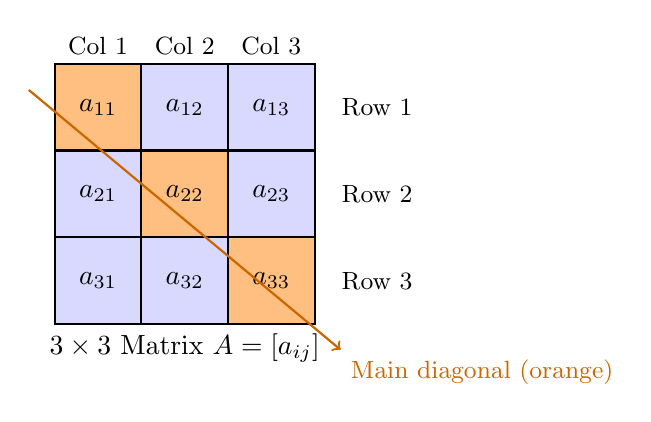
\begin{tikzpicture}[scale=1.1]
  \foreach \i in {1,2,3}{
    \foreach \j in {1,2,3}{
      \pgfmathsetmacro{\mycolor}{(\i==\j)?"orange!50":"blue!15"}
      \fill[\mycolor] (\j-1,4-\i) rectangle (\j,5-\i);
      \draw[thick] (\j-1,4-\i) rectangle (\j,5-\i);
      \node at (\j-0.5, 4.5-\i) {$a_{\i\j}$};
    }
  }
  \node[below] at (1.5,1) {$3\times3$ Matrix $A = [a_{ij}]$};
  \node[right] at (3.2,3.5) {\small Row 1};
  \node[right] at (3.2,2.5) {\small Row 2};
  \node[right] at (3.2,1.5) {\small Row 3};
  \node[above] at (0.5,4) {\small Col 1};
  \node[above] at (1.5,4) {\small Col 2};
  \node[above] at (2.5,4) {\small Col 3};
  \draw[->, thick, orange!80!black] (-0.3,3.7) -- (3.3,0.7) node[below right] {\small Main diagonal (orange)};
\end{tikzpicture}
\end{center}
The orange cells ($a_{11}, a_{22}, a_{33}$) form the main diagonal; blue cells are off-diagonal entries.

\medskip
\textbf{Visual 2: Linear Transformation --- Unit Square to Parallelogram}

\begin{center}
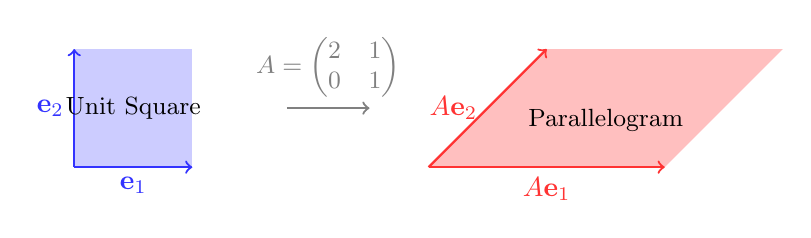
\begin{tikzpicture}[scale=1.5]
  \fill[blue!20] (0,0) -- (1,0) -- (1,1) -- (0,1) -- cycle;
  \draw[->, blue!80, thick] (0,0) -- (1,0) node[midway, below] {$\mathbf{e}_1$};
  \draw[->, blue!80, thick] (0,0) -- (0,1) node[midway, left] {$\mathbf{e}_2$};
  \node at (0.5,0.5) {\small Unit Square};
  \draw[->, thick, black!50] (1.8,0.5) -- (2.5,0.5) node[midway,above] {\small $A = \begin{pmatrix}2&1\\0&1\end{pmatrix}$};
  \fill[red!25] (3,0) -- (5,0) -- (6,1) -- (4,1) -- cycle;
  \draw[->, red!80, thick] (3,0) -- (5,0) node[midway, below] {$A\mathbf{e}_1$};
  \draw[->, red!80, thick] (3,0) -- (4,1) node[midway, left] {$A\mathbf{e}_2$};
  \node at (4.5,0.4) {\small Parallelogram};
\end{tikzpicture}
\end{center}
The matrix $A = \begin{pmatrix} 2 & 1 \\ 0 & 1 \end{pmatrix}$ shears the unit square (blue) into a parallelogram (red). The column vectors of $A$ are exactly the images of the standard basis vectors.

\medskip
\textbf{Visual 3: Symmetric vs Skew-Symmetric Matrices}

\begin{center}
\begin{tikzpicture}[scale=0.9]
  % Symmetric matrix
  \node[above] at (1.5,4.2) {\textbf{Symmetric}: $a_{ij} = a_{ji}$};
  \foreach \i/\j/\val in {1/1/4,1/2/3,1/3/1,2/1/3,2/2/2,2/3/5,3/1/1,3/2/5,3/3/7}{
    \pgfmathsetmacro{\myc}{(\i==\j)?"yellow!60":(((\i==1)&&(\j==2))||((\i==2)&&(\j==1)))?"green!40":(((\i==1)&&(\j==3))||((\i==3)&&(\j==1)))?"cyan!40":"magenta!30"}
    \fill[\myc] (\j-1,4-\i) rectangle (\j,5-\i);
    \draw[thick] (\j-1,4-\i) rectangle (\j,5-\i);
    \node at (\j-0.5, 4.5-\i) {\val};
  }
  % Skew-symmetric matrix
  \node[above] at (6.5,4.2) {\textbf{Skew-Symmetric}: $a_{ij} = -a_{ji}$};
  \foreach \i/\j/\val in {1/1/0,1/2/3,1/3/-1,2/1/-3,2/2/0,2/3/2,3/1/1,3/2/-2,3/3/0}{
    \pgfmathsetmacro{\myc}{(\i==\j)?"red!50":"blue!20"}
    \fill[\myc] (\j+4,4-\i) rectangle (\j+5,5-\i);
    \draw[thick] (\j+4,4-\i) rectangle (\j+5,5-\i);
    \node at (\j+4.5, 4.5-\i) {\val};
  }
  \node[below, red] at (6.5,0.9) {\small Diagonal = 0 (red)};
\end{tikzpicture}
\end{center}
In the symmetric matrix, matching-colour off-diagonal pairs are equal. In the skew-symmetric matrix, off-diagonal pairs are negatives of each other, and the diagonal (red) is forced to be zero.

\medskip
\textbf{Visual 4: Transpose Operation Diagram}

\begin{center}
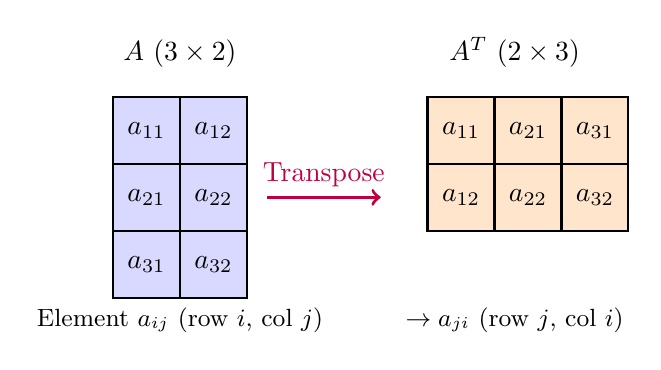
\begin{tikzpicture}[scale=0.85]
  % Matrix A (3x2)
  \node[above] at (1,3.3) {$A$ ($3\times2$)};
  \foreach \i/\j/\val in {1/1/{$a_{11}$},1/2/{$a_{12}$},2/1/{$a_{21}$},2/2/{$a_{22}$},3/1/{$a_{31}$},3/2/{$a_{32}$}}{
    \fill[blue!15] (\j-1,3-\i) rectangle (\j,4-\i);
    \draw[thick] (\j-1,3-\i) rectangle (\j,4-\i);
    \node at (\j-0.5, 3.5-\i) {\val};
  }
  \draw[->, very thick, purple] (2.3,1.5) -- (4.0,1.5) node[midway,above] {Transpose};
  % Matrix A^T (2x3)
  \node[above] at (6,3.3) {$A^T$ ($2\times3$)};
  \foreach \i/\j/\val in {1/1/{$a_{11}$},1/2/{$a_{21}$},1/3/{$a_{31}$},2/1/{$a_{12}$},2/2/{$a_{22}$},2/3/{$a_{32}$}}{
    \fill[orange!20] (\j+3.7,3-\i) rectangle (\j+4.7,4-\i);
    \draw[thick] (\j+3.7,3-\i) rectangle (\j+4.7,4-\i);
    \node at (\j+4.2, 3.5-\i) {\val};
  }
  \node[below] at (1,0) {\small Element $a_{ij}$ (row $i$, col $j$)};
  \node[below] at (6,0) {\small $\to a_{ji}$ (row $j$, col $i$)};
\end{tikzpicture}
\end{center}
The transpose maps $a_{ij} \to a_{ji}$: every row of $A$ becomes a column of $A^T$, and the order changes from $3\times2$ to $2\times3$.

%===========================================================
\section{Step-by-Step Algorithmic Workflows}
%===========================================================

\begin{learnbox}{Algorithm 1: Classify a Matrix}
\textbf{Input:} A matrix $A$ of order $m \times n$.
\begin{enumerate}
  \item Check order: Is $m = n$? If No $\to$ \textbf{Rectangular}. If Yes $\to$ proceed.
  \item Check for all-zero entries: Is every $a_{ij} = 0$? If Yes $\to$ \textbf{Zero/Null Matrix}. If No $\to$ proceed.
  \item Check diagonal: Are all off-diagonal entries zero? If Yes $\to$ Check if all diagonal entries equal: Yes $\to$ \textbf{Scalar}; No $\to$ \textbf{Diagonal}.
  \item Check triangularity: All entries below diagonal zero? $\to$ \textbf{Upper Triangular}. All above diagonal zero? $\to$ \textbf{Lower Triangular}.
  \item Check symmetry: Is $A^T = A$ (i.e., $a_{ij} = a_{ji}$)? Yes $\to$ \textbf{Symmetric}. Is $A^T = -A$? Yes $\to$ \textbf{Skew-Symmetric}.
  \item Check orthogonality: Is $A^T A = I$? Yes $\to$ \textbf{Orthogonal}.
  \item Check idempotency: Compute $A^2$. Is $A^2 = A$? Yes $\to$ \textbf{Idempotent}.
  \item Check involutory: Is $A^2 = I$? Yes $\to$ \textbf{Involutory}.
  \item Check nilpotency: Compute $A^2, A^3, \ldots$. Is $A^k = O$ for some $k$? Yes $\to$ \textbf{Nilpotent} with index $k$.
  \item If none of the above $\to$ \textbf{General Square Matrix}.
\end{enumerate}
\end{learnbox}

\begin{learnbox}{Algorithm 2: Compute Matrix Inverse (Adjugate Method)}
\textbf{Input:} Square matrix $A$ of order $n$.
\begin{enumerate}
  \item Compute $\det(A)$ by cofactor expansion. If $\det(A) = 0$, \textbf{stop} --- $A$ is singular (no inverse).
  \item Compute all $n^2$ cofactors: $C_{ij} = (-1)^{i+j} M_{ij}$ where $M_{ij}$ is the $(n-1)\times(n-1)$ minor determinant.
  \item Build the cofactor matrix $[C_{ij}]$.
  \item Transpose the cofactor matrix to get $\text{adj}(A) = [C_{ij}]^T$.
  \item Compute $A^{-1} = \dfrac{\text{adj}(A)}{\det(A)}$.
  \item Verify: compute $A \cdot A^{-1}$ and confirm all entries match $I_n$.
\end{enumerate}
\end{learnbox}

\begin{learnbox}{Algorithm 3: Decompose into Symmetric + Skew-Symmetric Parts}
\textbf{Input:} Square matrix $A$ of order $n$.
\begin{enumerate}
  \item Compute $A^T$ by interchanging rows and columns.
  \item Symmetric part: $P = \dfrac{A + A^T}{2}$. Verify $P^T = P$.
  \item Skew-symmetric part: $Q = \dfrac{A - A^T}{2}$. Verify $Q^T = -Q$ and all diagonal entries of $Q$ are zero.
  \item Confirm: $P + Q = A$.
\end{enumerate}
\end{learnbox}

\begin{learnbox}{Algorithm 4: Verify Transpose Properties}
\textbf{Input:} Matrices $A$, $B$ (conformable), scalar $k$.
\begin{enumerate}
  \item Property 1: Compute $(A^T)^T$ and verify it equals $A$.
  \item Property 2: Compute $(A+B)^T$ and $A^T + B^T$ independently; confirm equality.
  \item Property 3: Compute $(AB)^T$ and $B^T A^T$ independently; confirm equality entry by entry.
  \item Property 4: Compute $(kA)^T$ and $kA^T$; confirm equality.
\end{enumerate}
\end{learnbox}

%===========================================================
\section{Fully Worked Step-by-Step Numerical Examples}
%===========================================================

Most worked examples are integrated in Section 3 alongside each sub-topic definition. The following provides additional consolidated examples for exam preparation.

\textbf{Consolidated Example 6.1 --- Full Symmetric Verification:}

Given $K = \begin{pmatrix} 4 & -1 & 0 \\ -1 & 4 & -1 \\ 0 & -1 & 4 \end{pmatrix}$, verify $K$ is symmetric and verify that $B^T B$ is symmetric for $B = \begin{pmatrix} 2 & 1 \\ 0 & 3 \\ 1 & 0 \end{pmatrix}$.

\textbf{Part 1:} $K^T = \begin{pmatrix}4&-1&0\\-1&4&-1\\0&-1&4\end{pmatrix} = K$. Confirmed symmetric.

\textbf{Part 2:} $B^T = \begin{pmatrix}2&0&1\\1&3&0\end{pmatrix}$.
\[
B^T B = \begin{pmatrix}2&0&1\\1&3&0\end{pmatrix}\begin{pmatrix}2&1\\0&3\\1&0\end{pmatrix} = \begin{pmatrix}4+0+1&2+0+0\\2+0+0&1+9+0\end{pmatrix} = \begin{pmatrix}5&2\\2&10\end{pmatrix}.
\]
$(1,2) = 2 = (2,1)$. Symmetric confirmed. \checkmark

\textbf{Consolidated Example 6.2 --- Full Skew-Symmetric Decomposition:}

Let $M = \begin{pmatrix}3&-4\\6&7\end{pmatrix}$. Decompose $M$ into symmetric and skew-symmetric parts.

$M^T = \begin{pmatrix}3&6\\-4&7\end{pmatrix}$.

Symmetric part: $P = \dfrac{M + M^T}{2} = \dfrac{1}{2}\begin{pmatrix}6&2\\2&14\end{pmatrix} = \begin{pmatrix}3&1\\1&7\end{pmatrix}$.

Skew part: $Q = \dfrac{M - M^T}{2} = \dfrac{1}{2}\begin{pmatrix}0&-10\\10&0\end{pmatrix} = \begin{pmatrix}0&-5\\5&0\end{pmatrix}$.

Verify diagonal of $Q$: both entries are $0$. \checkmark \quad Verify $Q^T = \begin{pmatrix}0&5\\-5&0\end{pmatrix} = -Q$. \checkmark

Verify: $P + Q = \begin{pmatrix}3&1\\1&7\end{pmatrix} + \begin{pmatrix}0&-5\\5&0\end{pmatrix} = \begin{pmatrix}3&-4\\6&7\end{pmatrix} = M$. \checkmark

%===========================================================
\section{Tabular Reference --- All Matrix Types}
%===========================================================

\begin{center}
\begin{tabular}{@{}p{2.8cm}p{4.2cm}p{3cm}p{4cm}@{}}
\toprule
\textbf{Matrix Type} & \textbf{Definition / Condition} & \textbf{Example} & \textbf{Engineering Occurrence} \\
\midrule
Square & $m = n$ & $\begin{pmatrix}1&2\\3&4\end{pmatrix}$ & Stiffness matrices in FEA \\
\addlinespace
Rectangular & $m \neq n$ & $\begin{pmatrix}1&2&3\\4&5&6\end{pmatrix}$ & Sensor data matrices \\
\addlinespace
Row Vector & $m = 1$ & $\begin{pmatrix}1&2&3\end{pmatrix}$ & State vector in control systems \\
\addlinespace
Column Vector & $n = 1$ & $\begin{pmatrix}1\\2\\3\end{pmatrix}$ & Force/displacement vector in FEA \\
\addlinespace
Zero Matrix & $a_{ij} = 0\ \forall\, i,j$ & $\begin{pmatrix}0&0\\0&0\end{pmatrix}$ & Initialised memory in simulation \\
\addlinespace
Identity & $a_{ii}=1$, $a_{ij}=0$ ($i\neq j$) & $\begin{pmatrix}1&0\\0&1\end{pmatrix}$ & No-op transformation in graphics \\
\addlinespace
Diagonal & $a_{ij}=0$ for $i\neq j$ & $\begin{pmatrix}3&0\\0&5\end{pmatrix}$ & Inertia tensors (principal axes) \\
\addlinespace
Scalar & $a_{ij} = c\,\delta_{ij}$ & $\begin{pmatrix}4&0\\0&4\end{pmatrix}$ & Uniform scaling in graphics \\
\addlinespace
Upper Triangular & $a_{ij}=0$ if $i > j$ & $\begin{pmatrix}1&2\\0&3\end{pmatrix}$ & LU factorisation (U factor) \\
\addlinespace
Lower Triangular & $a_{ij}=0$ if $i < j$ & $\begin{pmatrix}1&0\\2&3\end{pmatrix}$ & LU factorisation (L factor) \\
\addlinespace
Symmetric & $A^T = A$ & $\begin{pmatrix}1&2\\2&5\end{pmatrix}$ & Stiffness/mass matrices in FEA \\
\addlinespace
Skew-Symmetric & $A^T = -A$; diag $= 0$ & $\begin{pmatrix}0&3\\-3&0\end{pmatrix}$ & Angular velocity tensor in robotics \\
\addlinespace
Orthogonal & $A^T A = I$ & $\begin{pmatrix}0&-1\\1&0\end{pmatrix}$ & Rotation matrices in 3D graphics \\
\addlinespace
\textbf{Idempotent} & $A^2 = A$; eigenvalues $\in\{0,1\}$ & $\begin{pmatrix}1&0\\0&0\end{pmatrix}$ & Projection operators in signal processing \\
\addlinespace
\textbf{Involutory} & $A^2 = I$; eigenvalues $\in\{-1,+1\}$ & $\begin{pmatrix}1&0\\0&-1\end{pmatrix}$ & Reflection matrices in computer graphics \\
\addlinespace
\textbf{Nilpotent} & $A^k = O$ for some $k \geq 1$; eigenvalues all $0$ & $\begin{pmatrix}0&1\\0&0\end{pmatrix}$ & Shift operators in signal processing; Jordan blocks \\
\bottomrule
\end{tabular}
\end{center}

%===========================================================
\section{Common Student Mistakes and Pitfalls}
%===========================================================

\begin{mistakebox}{Common Mistakes in Matrix Fundamentals}
\begin{tabular}{@{}p{3.5cm}p{5cm}p{6cm}@{}}
\toprule
\textbf{Mistake} & \textbf{Why Students Make It} & \textbf{Correct Approach} \\
\midrule
Confusing $a_{ij}$ with $a_{ji}$ & Row and column subscripts look interchangeable & $a_{ij}$ is row $i$, column $j$ --- always row first. $a_{23}$ is row 2, column 3. \\
\addlinespace
Assuming all square matrices have an inverse & Every number (except 0) has a reciprocal, so the analogy breaks & Compute $\det(A)$ first. If $\det(A) = 0$, the matrix is singular and has no inverse. \\
\addlinespace
Writing $AB = BA$ (commutativity error) & Multiplication of numbers is commutative; students apply the same rule to matrices & Always verify with explicit computation. $AB \neq BA$ in general. Counterexample in Example 1.3 above. \\
\addlinespace
Writing $(AB)^T = A^T B^T$ (wrong transpose order) & Students forget the order reversal rule & The correct rule is $(AB)^T = B^T A^T$. Order \emph{reverses}. \\
\addlinespace
Forgetting to transpose the cofactor matrix to get adj$(A)$ & Students compute the cofactor matrix and use it directly & adj$(A) = (\text{cofactor matrix})^T$. You must transpose first. \\
\addlinespace
Thinking a matrix with equal elements is symmetric & ``Symmetric'' sounds like ``has repeated values'' & Symmetric means $a_{ij} = a_{ji}$ (mirror across diagonal), not repeated row or column entries. \\
\addlinespace
Assuming skew-symmetric diagonal can be nonzero & No explicit condition seems to restrict the diagonal at first glance & Proof: $a_{ii} = -a_{ii} \Rightarrow a_{ii} = 0$. All diagonal entries of skew-symmetric matrices are \emph{always} zero. \\
\addlinespace
Confusing Idempotent ($A^2 = A$) with Involutory ($A^2 = I$) & Both involve squaring a matrix and comparing with a ``special'' matrix & Idempotent compares with $A$ itself; Involutory compares with the identity $I$. These are completely different conditions. \\
\bottomrule
\end{tabular}
\end{mistakebox}

%===========================================================
\section{Comprehensive Assessment Suite}
%===========================================================

\subsection*{Viva-Voce Questions}

\begin{enumerate}
  \item \textbf{[Sub-topic 1]} What is the order of a matrix? What does the notation $a_{23}$ mean? If $a_{23} = 5$, where exactly is this entry located?
  \item \textbf{[Sub-topic 2]} Define Idempotent, Involutory, and Nilpotent matrices with their algebraic conditions. Give one concrete $2\times2$ example for each. What are the eigenvalue constraints for each type?
  \item \textbf{[Sub-topic 3]} Why is matrix multiplication not commutative? Provide a specific counterexample using $2 \times 2$ matrices.
  \item \textbf{[Sub-topic 3]} State the conformability condition for the product $AB$ to exist. If $A$ is $3 \times 4$ and $B$ is $4 \times 5$, what is the order of $AB$?
  \item \textbf{[Sub-topic 4]} State all four properties of the transpose operation. Which property involves a reversal of order, and why?
  \item \textbf{[Sub-topic 5]} What condition must a matrix satisfy to have an inverse? State the formula $A^{-1}$ in terms of the adjugate. State $(AB)^{-1}$ in terms of $A^{-1}$ and $B^{-1}$.
  \item \textbf{[Sub-topic 5]} If we must solve $A\mathbf{x} = \mathbf{b}$, why do we write $\mathbf{x} = A^{-1}\mathbf{b}$ and not $\mathbf{x} = \mathbf{b} A^{-1}$?
  \item \textbf{[Sub-topic 6]} Can a rectangular matrix be symmetric? Justify your answer with reference to the definition.
  \item \textbf{[Sub-topic 7]} Prove that all diagonal entries of a skew-symmetric matrix must be zero. Start from the definition $A^T = -A$ and set $i = j$.
\end{enumerate}

\subsection*{Descriptive Exam Questions}

\begin{enumerate}
  \item Classify and justify the types of the following six matrices: $\begin{pmatrix}1&0\\0&1\end{pmatrix}$, $\begin{pmatrix}0&1\\0&0\end{pmatrix}$, $\begin{pmatrix}1&0\\0&-1\end{pmatrix}$, $\begin{pmatrix}1&0\\0&0\end{pmatrix}$, $\begin{pmatrix}3&0\\0&5\end{pmatrix}$, $\begin{pmatrix}0&2\\-2&0\end{pmatrix}$. For any Idempotent, Involutory, or Nilpotent matrices, verify the algebraic condition by computing the required matrix power step by step.
  \item Given $A = \begin{pmatrix}1&2\\3&4\end{pmatrix}$ and $B = \begin{pmatrix}0&1\\1&0\end{pmatrix}$: compute $AB$, $BA$, $(AB)^T$, and verify the reversal rule $(AB)^T = B^T A^T$ by computing both sides independently.
  \item Find the inverse of $A = \begin{pmatrix}3&1&2\\0&2&1\\1&0&3\end{pmatrix}$ using the adjugate method. Show all nine cofactors individually, build adj$(A)$, divide by $\det(A)$, and verify $A \cdot A^{-1} = I$.
  \item For $A = \begin{pmatrix}5&-2&4\\3&0&1\\-1&6&2\end{pmatrix}$, decompose $A$ into its symmetric and skew-symmetric parts. Verify the diagonal of the skew-symmetric part is zero, verify $S^T = -S$, and confirm $A = P + Q$.
  \item Prove from first principles that $(AB)^T = B^T A^T$. Start from the definition of matrix multiplication and the definition of transpose, and derive the result for general $m \times n$ matrix $A$ and $n \times p$ matrix $B$.
\end{enumerate}

\subsection*{Multiple Choice Questions (MCQs)}

\textbf{MCQ 1 [Sub-topic 1]:} If $A = [a_{ij}]$ is a matrix of order $3 \times 5$, what is $a_{24}$?
\begin{enumerate}[label=(\Alph*)]
  \item The element in row 4, column 2
  \item \textbf{The element in row 2, column 4}
  \item The element in row 2, column 4 only if the matrix is square
  \item The element on the main diagonal
\end{enumerate}
\textit{Explanation:} $a_{ij}$ always means row $i$, column $j$. So $a_{24}$ is row 2, column 4, regardless of whether the matrix is square.

\medskip
\textbf{MCQ 2 [Sub-topic 2 --- Idempotent/Involutory/Nilpotent Distinction]:} Which of the following correctly distinguishes Idempotent, Involutory, and Nilpotent matrices?
\begin{enumerate}[label=(\Alph*)]
  \item Idempotent: $A^2 = I$; Involutory: $A^2 = A$; Nilpotent: $A^k = I$
  \item Idempotent: $A^2 = 0$; Involutory: $A^2 = A$; Nilpotent: $A^k = I$
  \item \textbf{Idempotent: $A^2 = A$; Involutory: $A^2 = I$; Nilpotent: $A^k = O$ for some positive integer $k$}
  \item Idempotent: $A^k = O$; Involutory: $A^2 = A$; Nilpotent: $A^2 = I$
\end{enumerate}
\textit{Explanation:} The definitions are distinct: Idempotent compares $A^2$ with $A$; Involutory compares $A^2$ with $I$; Nilpotent reaches the zero matrix after some power $k$.

\medskip
\textbf{MCQ 3 [Sub-topic 3]:} What is the order of $AB$ if $A$ is $4 \times 3$ and $B$ is $3 \times 6$?
\begin{enumerate}[label=(\Alph*)]
  \item $3 \times 3$
  \item $4 \times 3$
  \item \textbf{$4 \times 6$}
  \item $3 \times 6$
\end{enumerate}
\textit{Explanation:} Conformability: $(m \times n)(n \times p) = m \times p$. So $(4 \times 3)(3 \times 6) = 4 \times 6$.

\medskip
\textbf{MCQ 4 [Sub-topic 4]:} Which of the following is the correct transpose property for a product?
\begin{enumerate}[label=(\Alph*)]
  \item $(AB)^T = A^T B^T$
  \item $(AB)^T = A B^T$
  \item $(AB)^T = A^T B$
  \item \textbf{$(AB)^T = B^T A^T$}
\end{enumerate}
\textit{Explanation:} The order \emph{reverses} when taking the transpose of a product: $(AB)^T = B^T A^T$.

\medskip
\textbf{MCQ 5 [Sub-topic 5]:} A matrix $A$ is invertible if and only if:
\begin{enumerate}[label=(\Alph*)]
  \item $A$ is symmetric
  \item $A$ is square
  \item \textbf{$\det(A) \neq 0$}
  \item $A$ has all positive entries
\end{enumerate}
\textit{Explanation:} A square matrix has an inverse precisely when its determinant is nonzero. Being square is necessary but not sufficient.

\medskip
\textbf{MCQ 6 [Sub-topic 6]:} Which statement about symmetric matrices is TRUE?
\begin{enumerate}[label=(\Alph*)]
  \item A rectangular matrix can be symmetric
  \item A symmetric matrix must have all equal entries
  \item \textbf{$A^T A$ is always symmetric for any matrix $A$}
  \item The diagonal entries of a symmetric matrix must be zero
\end{enumerate}
\textit{Explanation:} $(A^T A)^T = A^T (A^T)^T = A^T A$, so $A^T A$ is always symmetric regardless of the shape of $A$.

\medskip
\textbf{MCQ 7 [Sub-topic 7]:} Which of the following is necessarily true for a skew-symmetric matrix $A$?
\begin{enumerate}[label=(\Alph*)]
  \item All entries are positive
  \item All entries are negative
  \item $A^T = A$
  \item \textbf{All diagonal entries are zero}
\end{enumerate}
\textit{Explanation:} From $A^T = -A$, setting $i = j$ gives $a_{ii} = -a_{ii}$, forcing $a_{ii} = 0$ for all $i$.

%===========================================================
\section{Quick Recap and Formula Sheet}
%===========================================================

\begin{learnbox}{Matrix Fundamentals --- Formula Sheet (10 Key Points)}
\begin{itemize}
  \item \textbf{Matrix order $m \times n$:} $m$ rows, $n$ columns; element $a_{ij}$ is in row $i$, column $j$ --- row first, column second, always.
  \item \textbf{Key special types:} Idempotent $A^2 = A$ (projection); Involutory $A^2 = I$ (reflection); Nilpotent $A^k = O$ (shift); Orthogonal $A^T A = I$ (rotation/reflection preserving length).
  \item \textbf{Multiplication conformability:} $AB$ exists iff inner dimensions match; $(m \times n)(n \times p) = m \times p$.
  \item \textbf{Non-commutativity:} $AB \neq BA$ in general; $(AB)C = A(BC)$ always (associativity holds).
  \item \textbf{Transpose reversal:} $(AB)^T = B^T A^T$; order reverses. Similarly $(A+B)^T = A^T + B^T$ and $(kA)^T = kA^T$.
  \item \textbf{Inverse formula:} $A^{-1} = \text{adj}(A) / \det(A)$; requires $\det(A) \neq 0$; adj$(A) = (\text{cofactor matrix})^T$.
  \item \textbf{Inverse reversal:} $(AB)^{-1} = B^{-1} A^{-1}$; $(A^T)^{-1} = (A^{-1})^T$; $(A^{-1})^{-1} = A$.
  \item \textbf{Symmetric condition:} $A^T = A \Leftrightarrow a_{ij} = a_{ji}$ for all $i, j$; $A$ must be square; $A^T A$ is always symmetric.
  \item \textbf{Skew-symmetric condition:} $A^T = -A \Leftrightarrow a_{ij} = -a_{ji}$; diagonal entries are \emph{always} zero.
  \item \textbf{Symmetric--skew decomposition:} Every square matrix $A = \dfrac{A + A^T}{2} + \dfrac{A - A^T}{2}$ (symmetric part + skew-symmetric part); the decomposition is unique.
\end{itemize}
\end{learnbox}

\end{document}
